%!TEX root = ..\lections.tex
Предыдущая лекция была посвящена исследованию состояний равновесия двумерных линейных систем. Было показано, что их характер может быть определен из анализа расположения корней характеристического уравнения на комплексной плоскости. Перейдем теперь к исследованию состояний равновесия нелинейных систем.

\section{Метод линеаризации}%
\label{sec:metod_linearizatsii}

Рассмотрим записанную в векторной форме нелинейную систему

\begin{equation}
        \label{eq:4.1}
        \dot{\vec x} = \vec F(\vec x), ~ \vec x \in \R^n, \vec F: \R^n \to \R^n,    
\end{equation}
где $\vec F(\vec x)$ -- гладкая вектор-функция. Предположим, что система \eqref{eq:4.1}  имеет состояние равновесия $\vec x = \vec x^*$. Введем малое возмущение $\vec \xi(t) = \vec x(t) - \vec x^*    $,
для которого из системы \eqref{eq:4.1} имеем
\begin{equation}
        \label{eq:4.2}
        \dot{\vec \xi} = \vec F( \vec x^* + \vec \xi).  
\end{equation}
Раскладывая правую часть системы \eqref{eq:4.2} в ряд Тейлора, получим
\begin{equation}
        \label{eq:4.3}
        \dot{\vec \xi} = \vec A \vec \xi + \dots,
\end{equation}
где $\vec A$ -- $n \times n$ -- матрица Якобы с элементами
\begin{equation}
        \label{eq:}
        a_{ik} = \pdv{F_i}{x_k} \eval_{x=x^*}.
\end{equation}
Отбросим в правой части \eqref{eq:4.3} все нелинейные по $\vec \xi$ слагаемые и рассмотрим систему
\begin{equation}
        \label{eq:4.4}
        \dot{\vec \xi} = \vec A \vec \xi.
\end{equation}
Переход от нелинейной системы \eqref{eq:4.3}  к линейной системе \eqref{eq:4.4} называется её линеаризацией. Мы не будем пока обсуждать соотношение между траекториями систем \eqref{eq:4.3} и \eqref{eq:4.4} , а рассмотрим возможные типы состояний равновесия линейной системы \eqref{eq:4.4} .

На предыдущих лекциях мы уже рассмотрели свойства системы \eqref{eq:4.4}  в одномерном и двумерном случаях. Как было показано, в этих случаях поведение траекторий зависит от корней характеристического уравнения. Аналогичным свойством обладает и система \eqref{eq:4.4} , в случае когда размерность её выше двух . Будем искать решение системы \eqref{eq:4.4} в виде
\begin{equation}
        \label{eq:4.5}
\vec \xi = \vec C e^{\lambda t},
\end{equation}
где $\vec C$ -- постоянная матрица столбец. Подстановка \eqref{eq:4.5} в \eqref{eq:4.4} приводит к системе линейных однородных уравнений, которая имеет нетривиальное решение, если 
\begin{equation}
        \label{eq:4.6}
        \det(\vec A - \lambda \vec E) =0,
\end{equation}
где $\vec  E$ -- единичная матрица. Уравнение \eqref{eq:4.6} эквивалентно алгебраическому уравнению
\begin{equation}
        \label{eq:4.7}
        a_0 \lambda^n + a` \lambda^{n-1} + \dots + a_n =0.
\end{equation}
Уравнение \eqref{eq:4.7} называется характеристическим, а его корни характеристическими показателями состояния равновесия $\vec x =\vec x^*$. 
Справедливы следующие, установленные А.М. Ляпуновым, утверждения:
\begin{itemize}
        \item Если корни уравнения \eqref{eq:4.7} имеют отрицательные вещественные части, т.е. $\Re \lambda_i < 0 ~ (i= 1,2,\dots,n)$, то состояние равновесия системы \eqref{eq:4.4} асимптотически устойчиво.
 \item Если среди корней уравнения \eqref{eq:4.7} есть хотя бы один с положительной вещественной частью, то состояние равновесия системы \eqref{eq:4.4} неустойчиво по Ляпунову.
 \item  Если уравнение \eqref{eq:4.7} не имеет корней с положительной вещественной частью, но имеет некоторое число корней с нулевой вещественной частью, то состояние равновесия системы \eqref{eq:4.4} может быть как устойчивым (но не асимптотически), так и неустойчивым.
\end{itemize}
Таким образом, вопрос об устойчивости состояний равновесия многомерных линейных систем сводится к исследованию характера корней алгебраического уравнения.

Вернемся теперь к исходной нелинейной системы \eqref{eq:4.1},
устойчивость состояний равновесия которой может быть установлена теоремами Ляпунова. Согласно теореме Ляпунова об устойчивости по первому приближению (так называемый первый метод Ляпунова), если корни уравнения \eqref{eq:4.7} удовлетворяют условию $\Re \lambda_i \neq 0~ (i=1,2,\dots,n)$, то характер устойчивости состояний равновесия нелинейной системы \eqref{eq:4.1} и соответствующей линеаризованной системы \eqref{eq:4.7} совпадают. Таким образом, состояние равновесия системы \eqref{eq:4.1} является асимптотически устойчивым, если $\Re \lambda_i<0~ (i=1,2,\dots,n) $ и неустойчивым если среди корней уравнений \eqref{eq:4.7} имеется хотя бы один с положительной вещественной частью.

\section{Критерий Рауса-Гурвица}%
\label{sec:4.2}

Из сказанного выше следует, что решение задачи об устойчивости
состояний равновесия нелинейных систем сводится к анализу расположения
корней характеристического уравнения на комплексной плоскости, т.е. к чисто
алгебраической задаче. Однако, в случае многомерных (размерности три и
выше) систем, как правило, найти характеристические показатели
$\lambda_i$ в явном
виде не удается. Поэтому были развиты критерии и методы, позволяющие
судить об устойчивости состояний равновесия без непосредственного решения
характеристического уравнения. Одним из наиболее известных таких критериев
является критерий Рауса-Гурвица.

Критерии устойчивости Рауса (Routg E.Y.) и Гурвица (Hurwitz A.), вошедших в виде единого критерия, были разработаны в конце 18-го века в связи с проблемами, возникающими в тот момент, в теории автоматического управления. Сформулируем этот критерий для уравнения \eqref{eq:4.7} с вещественными коэффициентами. Без ограничения общности будем считать, что коэффициент $a_0$ является положительным. Составим из коэффициентов $a_j ~ (j=0,1,2,\dots,n)$ квадратную матрицу размерности $n\times n$ в соответствии со следующими правилами:
\begin{itemize}
        \item Первая строка матрицы состоит из коэффициентов с нечетными индексами, начиная с $a_1$.
        \item Элементы каждой последующей строки образуются из соответствующих элементов предшествующей строки уменьшением индексов на единицу.
        \item Если при таком построении индекс $k$ какого-либо коэффициента $a_k$ превосходит значение $n$ или становится отрицательным, то он приравнивается нулю, т.е. $a_k=0$. 
\end{itemize}

В результате описанной процедуры получится $n\times n$ матрица следующего вида
\begin{equation}
        \label{eq:}
        \vec{A_R} = 
        \begin{pmatrix}
                a_1 & a_3 & a_5 & \dots & 0 & 0 \\
                a_0 & a_2 & a_4 & \dots & 0 & 0 \\
                0 & a_1 & a_3 & \dots & 0 & 0 \\
                0 & a_0 & a_2 & \dots & 0 & 0 \\
                \dots & \dots & \dots & \dots & a_{n-1} & 0 \\
                0 & 0 &0 & \dots & a_{n-2} & a_n \\
        \end{pmatrix}
\end{equation}
Заметим, что на главной диагонали матрицы $\vec{A_R}$ стоят последовательно все коэффициенты уравнения \eqref{eq:4.7}, начиная с $a_1$. Далее, выпишем все главные диагональные миноры матрицы $\vec{A_R}$ 
\begin{equation}
        \label{eq:4.8}
        \Delta_1 = a_1, ~ 
        \Delta_2 = 
        \begin{vmatrix}
                a_1 & a_3 \\
                a_0 & a_2
        \end{vmatrix}, ~ 
        \dots, ~
        \Delta_n = a_n \Delta_{n-1}.
\end{equation}

Критерий Рауса-Гурввица состоит в следующем. Для того, чтобы все корни уравнения \eqref{eq:4.7} с вещественными коэффициентами и $a_0>0$ имели отрицательные вещественные части, необходимо и достаточно, чтобы все главные диагональные миноры были положительны
\begin{equation}
        \label{eq:4.9}
        \Delta_n > 0,~\Delta_2> 0, ~ \dots,~\Delta_{n-1}>0,~\Delta_n >0.
\end{equation}

Таким образом, условия \eqref{eq:4.9} гарантируют асимптотическую устойчивость состояния равновесия линейной \eqref{eq:4.4} и нелинейной \eqref{eq:4.1} систем. Однако заметим, что в случае нелинейной системы \eqref{eq:4.1} это лишь локальная устойчивость в малой окрестности состояния равновесия.

В качестве примера применения критерия Рауса-Гурвица рассмотрим уравнение \eqref{eq:4.7} в случае $n=3$. Для удобства перепишем это уравнение в следующем эквивалентном виде
\begin{equation}
        \label{eq:4.10}
        \lambda^3 - a \lambda^2 + b \lambda +c =0
\end{equation}
где
\begin{equation}
        \label{eq:}
        a= \frac{a_1}{a_0}, ~ b= \frac{a_2}{a_0}, ~ c= \frac{a_3}{a_0}.
\end{equation}
Введем, отвечающую уравнению \eqref{eq:4.10}, матрицу
\begin{equation}
        \label{eq:}
        \vec{A_R} = 
        \begin{pmatrix}
                a & c & 0 \\
                1 & b & 0 \\
                0 & a & c \\    
        \end{pmatrix}
        .
\end{equation}
Легко видеть, что главные диагональные миноры этой матрицы имеют вид
\begin{equation}
        \label{eq:4.11}
        \Delta_1 = a, ~ \Delta_2 = ab - c, ~ \Delta_3= c(ab-c).
\end{equation}
Отсюда, согласно критерию Рауса-Гурвица, все корни уравнения \eqref{eq:4.10} имеют отрицательные вещественные части, если параметры этого уравнения удовлетворяют неравенствам
\begin{equation}
        \label{eq:4.12}
        a>0, \quad ab-c>0, \quad c>0.
\end{equation}

\section{Второй метод Ляпунова}%
\label{sec:4.3}

Рассмотрим еще один метод, позволяющий устанавливать условия
устойчивости состояний равновесия без непосредственного нахождения
характеристических показателей. А.М. Ляпуновым была развита теория, в
основе которой лежит построение специальных функций, позволяющих, в
случае их существования, судить об устойчивости и неустойчивости состояний
равновесия. Эти функции получили название функций Ляпунова, а
базирующаяся на них теория устойчивости -- второго метода Ляпунова.
Изложим кратко основные идеи этого метода для автономных систем.

Рассмотрим скалярную функцию $V(x_1,x_2,\dots,x_n)$ или в векторном виде $V(\vec x)$, определенную в фазовом пространстве системы \eqref{eq:4.1}, непрерывную в некоторой области $D$, содержащей состояние равновесия $\vec x= \vec x^*$. Кроме того, предположим, что $V(\vec x)$ имеет в $D$ непрерывные частные производны. В основе второго метода Ляпунова лежит использование свойств так называемых 
\textbf{знакоопределенных и знакопостоянных} функций.
\begin{enumerate}
        \item Функция $V(\vec x)$ называется знакоопределенной в области $D$, если она обращается в нуль лишь в состоянии равновесия и принимает значения одного знака во всех остальных точках области $D$. Очевидно, что знакоопределенные функции бывают двух типов -- положительно и отрицательно определенные. 
        \item Функция $V(\vec x)$ называется знакопостояннной в области $D$, если она обращается в нуль не только в состоянии равновесия, но и в некоторых других точках области $D$, и имеет значения только одного знака во всех остальных точках области $D$.
\end{enumerate}

Поясним смысл этих определений. Рассмотрим функции
\begin{equation}
        \label{eq:}
        \begin{gathered}
        V_1( x_1, x_2,x_3) = x_1^2 +x_2^2 +x_3^2, \\
        V_2(x_1,x_2,x_3)= (x_1+x_3)^2 +x_2^2.
        \end{gathered}
\end{equation}
Очевидно, что функция $V_1$ является положительно определенной в области $D= \R^3$, а функция $V_2$-- знакоположительной, поскольку она обращается в нуль не только в точке $x_1=x_2=x_3$, но и при $x_2=0, ~ x_3=-x_1$.

Во втором методе Ляпунова задача об устойчивости состояний равновесия решается с помощью изучения поведения функции $V(\vec x)$ вдоль траектории системы \eqref{eq:4.1}. Рассмотрим структуру поверхностей уровня $V(\vec x) = C= \const$ знакоопределенных функций, которую определяет следующее утверждение.

Если функций $V(\vec x)$ является знакоопределенной, то существует такое положительное число $C^*$, что все поверхности уровня $V(\vec x)=C$, где $\abs{C} < C^*$ являются замкнутыми относительно точки $x=x^*$. 

Заметим, что поверхности $V(\vec x) = C$ называется замкнутой, если на любой непрерывной линии, соединяющей точку $\vec x = \vec x^*$ с точкой границы области $D$, существует по крайней мере одна точка, в которой $V(\vec x) =C$. Поясним свойства поверхностей уровня знакоопределенных функций на примере положительно определенных функций. На рис.\ref{fig:4.1}a представлен пример простейшей положительно определенной функции двух переменных. В этом примере ясно представлены основные свойства поверхностей уровня положительно определенных функций: они замкнуты, не имеют общих точек
, окружают точку $\vec x = \vec x^* =0$ и стягиваются к ней при $C \to 0$.

\begin{figure}[h!]
        \centering
        \begin{minipage}{0.45\linewidth}
                \centering  
                
\includegraphics[]{fig/lect4/1a}

                (a)
        \end{minipage}
        \begin{minipage}{0.45\linewidth}
                \centering  
                
\includegraphics[]{fig/lect4/1b}

                (b)      
        \end{minipage}
        \caption{Качественный вид положительно определенной функции двух переменных и линий уровня этой функции (a) и ориентация траекторий системы \eqref{eq:4.1} на поверхностях уровня $C_2 >C_1$ функции Ляпунова при выполнении теоремы об асимптотической устойчивости (b).}
        \label{fig:4.1}
\end{figure}

Поведение поверхностей уровня функции $V(\vec x)$ вдоль траектории системы \eqref{eq:4.1} может быть установлено с помощью производной по времени этой функции, вычисленной в сите системы \eqref{eq:4.1}. Такая производная находится следующим образом
\begin{equation}
        \label{eq:4.13}
        \dot V = \sum\limits_{i=1}^{n}  \pdv{V}{x_i} \dot x_{i} = \sum\limits_{i=1}^{n} \pdv{V}{x_{i}} F_i = 
        \qty( \grad V \cdot F),
\end{equation}
где круглые скобки означают скалярное произведение векторов. Заметим, что из \eqref{eq:4.13} вытекает условие $\dot V(\vec x)=0$, если $\vec x = \vec x^*$.

Сформулируем теперь теоремы Ляпунова, дающие достаточные условия устойчивости состояний равновесия.

\paragraph{Теорема об устойчивости.}%
\label{par:teorema_ob_ustoichivosti_}

Если для системы \eqref{eq:4.1} существует в области $D$
\textbf{знакоопределенная} функция $V(\vec x)$, является \textbf{знакопостоянной} 
функцией, знака противоположному знаку функции $V(\vec x)$, то состояние равновесия $\vec x = \vec x^*$ устойчиво в смысле Ляпунова.

\paragraph{Теорема об асимптотической устойчивости.}%
\label{par:teorema_ob_asimptoticheskoi_ustoichivosti}

Если для системы \eqref{eq:4.1} существует \textbf{знакоопределенная} функция $V(\vec x)$, производная которой по времени $\dot V$, вычисленная в силу этой системы, является также \textbf{ знакоопределенной}, знака противоположному знаку $V(\vec x)$, то состояние равновесия $\vec x= \vec x^*$ будет асимптотически устойчивым. 

Поясним геометрический смысл теоремы об асимптотической устойчивости. Пусть для определенности функция $V(\vec x)$ будет положительно, а 
$\dot V(\vec x)$ -- отрицательно определенными функциями. Неравенство $\dot V(\vec x)<0$ означает, что траектории системы \eqref{eq:4.1} в точках поверхности $V(\vec x)= C$ переходят снаружи внутрь, т.е. в направлении противоположном направлению вектора $\grad V$ (рис.\ref{fig:4.1}б). Отсюда, поскольку при $C \to 0$ поверхности $V(\vec x) = C$ стягиваются в точку $\vec x = \vec x^*$,следует, что любая траектории системы \eqref{eq:4.1} будет асимптотически приближаться к состоянию равновесия, пересекая каждую из поверхностей $V(\vec x) = C$ в одну и ту же сторону.
Это означает, что состояние равновесия $\vec x = \vec x^*$ является асимптотически устойчивым, а поверхность уровня $V(\vec x) = C_{max}$, соответствующая наибольшему значению константы $C$, при которой условия теоремы выполняются, выделяет в фазовом пространстве область, принадлежащую области притяжения состояния равновесия. Заметим, если, $C_{max} \to \infty$, то состояние равновесия является асимптотически устойчивым при любых начальных условиях, т.е. устойчивым в целом.

\paragraph{Пример.}%
\label{par:primer_}

Рассмотрим систему уравнений
\begin{equation}
        \label{eq:4.14old}
        \begin{cases}
                \dot x_1 = -x_1+x_2- x_1^3, \\
                \dot x_2 = -x_1 - x_2 - x_2^3.
        \end{cases}
\end{equation}
Нетрудно видеть, что система \eqref{eq:4.14} имеет единственное состояние равновесия в начале координат -- $O(x_1=x_2=0)$. Введем в рассмотрение положительно определенную функцию
\begin{equation}
        \label{eq:}
        V(x_1,x_2) = \frac{x_1^2}{2} + \frac{x_2^2}{2}
\end{equation}
и вычислим её производную в силу системы \eqref{eq:4.14old}
\begin{equation}
        \label{eq:4.15old}
       \dot V = x_1 \cdot \dot x_1 + x_2 \cdot \dot x_2 = -x_1^2 - x_2^2 - x_1^4 - x_2^4 \leq 0. 
\end{equation}
В силу \eqref{eq:4.15old} $\dot V( x_1,x_2)$ -- отрицательно определенная функция во всех точках фазовой плоскости, отличных от состояния равновесия $O$. Следовательно, $V(x_1,x_2)$-- функция Ляпунова и состояние равновесия
$O$ является асимптотически устойчивым в целом.
Заметим, что с помощью метода линеаризации можно было бы установить устойчивость состояния равновесия $O$ лишь в малом.

Таким образом, второй метод Ляпунова является эффективным способом
изучения устойчивости состояний равновесия нелинейных систем не только в
малом, но и в большом. Этот метод может быть также применен к системам с
угловыми координатами. Для таких систем из существования функции
Ляпунова, периодической по угловым координатам, вытекает глобальная
асимптотическая устойчивость системы (см. лекцию \ref{lect11}). Однако, к сожалению,
не существует стандартных способов построения функций Ляпунова для
нелинейных систем и, как правило, каждая система требует своего
индивидуального подхода. Наиболее часто функции Ляпунова ищутся в виде
квадратичных форм переменных исследуемых систем.

Обратим также внимание ещё на одно важное свойство поверхностей уровня знакоопределенных функций. Поверхность, на которой производная $\dot V$ в силу системы \eqref{eq:4.1} является знакоопределенной, называется \textbf{поверхностью без контакта}.
В некоторых случаях с помощью таких поверхностей можно получить ряд полезных свойств о поведении траекторий системы \eqref{eq:4.1} в фазовом пространстве, хотя при этом функция Ляпунова не существует. Например, выделить в фазовом пространстве так называемую поглощающую область (см. лекцию \ref{lect1}), оценить локализацию аттракторов и др.

\section{Грубые состояния равновесия трехмерных систем}%
\label{sec:4.4}

Метод линеаризации позволяет установить локальную устойчивость или
неустойчивость грубых состояний равновесия нелинейных систем, но ничего не
говорит о том, каким образом траектории приближаются к состоянию
равновесия или удаляются от него. Для понимания этих свойств исследуем
структуру разбиения фазового пространства на траектории в окрестности
состояний равновесия трехмерных систем. Следуя методу линеаризации,
рассмотрим сначала линейную систему \eqref{eq:4.4}. Предположим, что среди
характеристических показателей состояния равновесия нет кратных и
$\Re \lambda_i \neq 0, ~ i = 1,2,3.$

\subsection{Действительные корни}%
\label{sub:4.4.1}

В этом случае линейной заменой переменных $\vec u = \vec H \vec \xi$, где $\vec H$ -- матрица $3 \times 3$, система \eqref{eq:4.4} может быть приведена к следующему виду
\begin{equation}
        \label{eq:4.14}
        \dot u_1 = \lambda_1 u_1, ~ \dot u_2 = \lambda_2 u_2,~ \dot u_3 = \lambda_3 u_3.
\end{equation}
Система \eqref{eq:4.14} -- нормальная форма уравнений для состояний равновесия с действительными различными характеристическими показателями линейных трехмерных систем. Общее решение системы \eqref{eq:4.14} имеет вид 
\begin{equation}
        \label{eq:4.15}
        u_1 = u_1^{0} e^{\lambda_1 t}, \quad u_2=u_2^{0} e^{\lambda_2t}, \quad u_3 = u_3^{0} e^{\lambda_3 t},
\end{equation}
где $u_i^0=\const$.

\subsubsection{Корни $\lambda_i $ одного знака}%
\label{ssub:4.4.1a}

\paragraph{Случай отрицательных корней.}%
\label{par:sluchai_otritsatel_nykh_kornei_}

Из \eqref{eq:4.15} следует, что в этом случае при любых начальных условиях при $t \to \infty$ траектории системы \eqref{eq:4.14} стремятся к состоянию равновесия $O (u_1=u_2=u_3=0)$, которое является асимптотически устойчивым и называется устойчивым узлом. Рассмотрим, как именно траектории в фазовом пространстве $\R^3$ подходят к точке $O$. Пусть для определенности $\lambda_i$ упорядочены следующим образом: $\lambda_3< \lambda_2< \lambda_1<0$. Прежде всего заметим,
что плоскость $\{ u_1 =0 \}$ инвариантна относительно системы \eqref{eq:4.14}, т.е. траектории системы \eqref{eq:4.14} с начальными условиями на этой плоскости целиком принадлежат ей. 
Поскольку $\lambda_3< \lambda_2<0$, траектории системы \eqref{eq:4.14} с на плоскости $\{ u_1 =0\}$   ведут себя аналогично траекториям устойчивого узла двумерных систем (см. лекцию \ref{lect3}, рис.\ref{fig:4.2}a). 
\begin{figure}[h!]
        \centering
        \begin{minipage}{0.45\linewidth}
                \centering  
                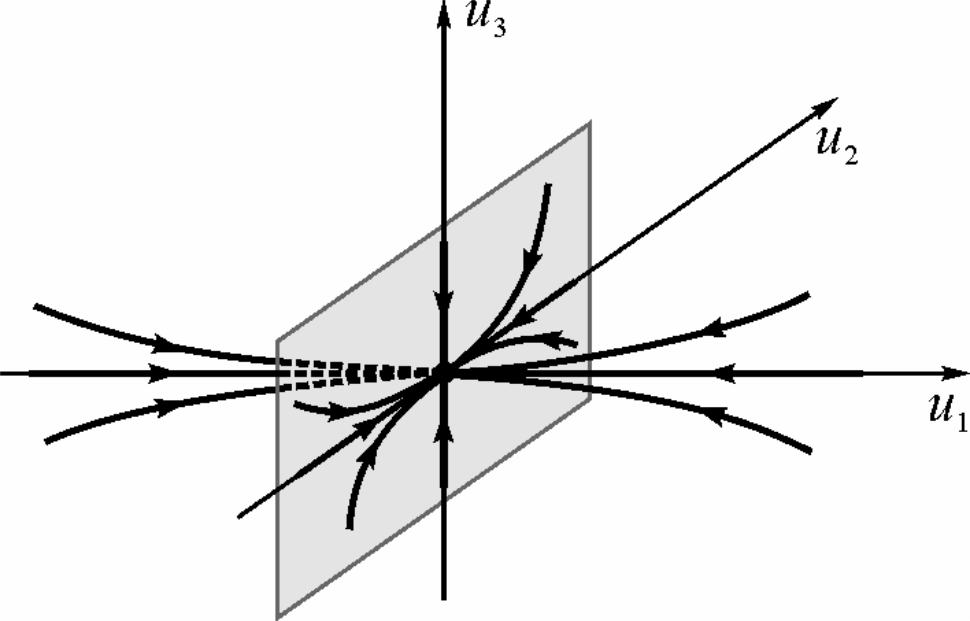
\includegraphics[]{fig/lect4/2a}

                (a)
        \end{minipage}
        \begin{minipage}{0.45\linewidth}
                \centering  
                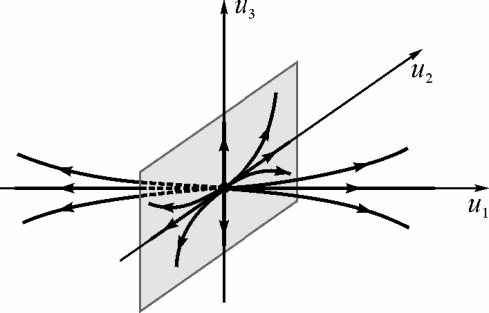
\includegraphics[]{fig/lect4/2b}

                (b)      
        \end{minipage}
        \caption{Состояние равновесия системы \eqref{eq:4.14}: устойчивый узел (a); неустойчивый узел (b). }
        \label{fig:4.2}
\end{figure}
Пусть теперь $u_1 \neq 0$. Из \eqref{eq:4.15} имеем
\begin{equation}
        \label{eq:4.16}
        \frac{u_{2}}{u_1} = \const \cdot e^{(\lambda_2-\lambda_1) t}, \quad \frac{u_3}{u_1}=\const \cdot e^{(\lambda_3 - \lambda_1) t}.
\end{equation}
В силу \eqref{eq:4.16} при $t \to \infty$ переменная $u_1 (t)$, при стремлении к состоянию равновесия $O$, убывает медленнее, чем переменные $u_2(t)$ и $u_3(t)$.
Следовательно, все траектории системы \eqref{eq:4.14}, за исключением траекторий плоскости $\{ u_1=u_2\}$, касаются в состоянии равновесия прямой $\{ u_2 = u_3 = 0 \}$, которая является ведущим направлением узла ( рис.\ref{fig:4.2}а).
\paragraph{Случай положительной корней.}%
\label{par:sluchai_polozhitel_noi_kornei_}

Пусть уравнение \eqref{eq:4.10} имеет только положительные корни, упорядоченные для определенности следующим образом: $\lambda_3 > \lambda_2>\lambda_1>0$. В силу \eqref{eq:4.15} все траектории системы \eqref{eq:4.14} покидают окрестность состояния равновесия $O$, которое в этом случае является неустойчивым и называется неустойчивым узлом. Поведение траекторий в окрестности неустойчивого узла устанавливается аналогично предыдущему случаю и показано на рис.\ref{fig:4.2}b.

\subsubsection{Корни $\lambda_i$ разного знака}%
\label{ssub:korni_lambda_i_raznogo_znaka}
\paragraph{Случай одного положительного и двух отрицательных корней.}%
\label{par:sluchai_odnogo_polozhitel_nogo_i_dvukh_otritsatel_nykh_kornei_}

Предположим, что уравнение \eqref{eq:4.10} имеет следующие корни: $\lambda_2<\lambda_1<0, ~ \lambda_3>0$. Непосредственно из системы \eqref{eq:4.14} следует, что все траектории с начальными условиями на плоскости $E^{s} = \qty{ (u_1,u_2) \in \R^2, ~ u_3 }$ целиком принадлежат этой плоскости, т.е. $E^s$ инвариантна относительно системы \eqref{eq:4.14}. Движения на плоскости $E^s$ определяются первыми двумя уравнениями системы \eqref{eq:4.14}, которые задают на ней устойчивый узел. При этом прямая 
$\qty{u_2=0}$ является ведущим, а прямая $\qty{u_1 = 0}$-- неведущими направлениями этого узла ( рис.\ref{fig:4.3}а). 

\begin{figure}[h!]
        \centering
        \begin{minipage}{0.45\linewidth}
                \centering  
                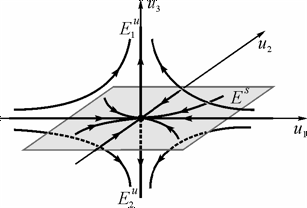
\includegraphics[]{fig/lect4/3a}

                (a)
        \end{minipage}
        \begin{minipage}{0.45\linewidth}
                \centering  
                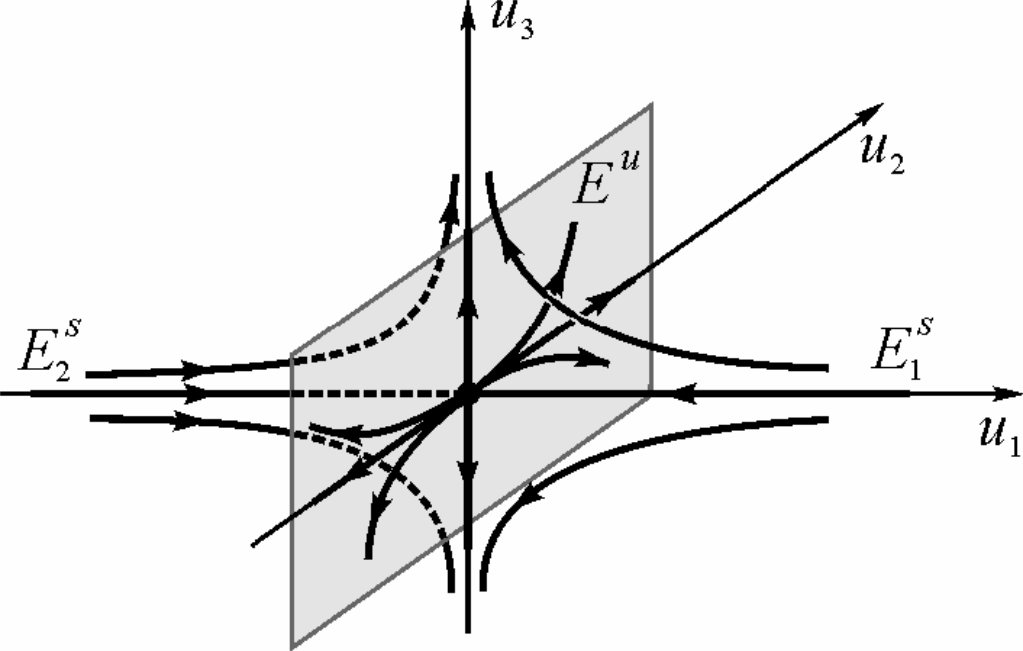
\includegraphics[]{fig/lect4/3b}

                (b)      
        \end{minipage}
        \caption{Состояния равновесия системы \eqref{eq:4.14}: седло с двумерным устойчивым и одномерным неустойчивым многообразиями (a); седло с двумерным неустойчивым и одномерным устойчивым многообразиями (b).}
        \label{fig:4.3}
\end{figure}

Очевидно, что прямая $E^u = \qty{u_1 = u_2 = 0, ~ u_3 \in \R}$ также инвариантна относительно системы \eqref{eq:4.14}. Движения на этой прямой определяются третьим уравнением системы \eqref{eq:4.14}. Поскольку $\lambda_3>0$, то для траектории системы \eqref{eq:4.14} с начальными условиями на этой прямой выполняется либо условие $u_3(t) \to \infty$, либо $u_3(t) \to -\infty$ ( рис.\ref{fig:4.3}а). Рассмотрим поведение траекторий с начальными условиями вне $E^s$ и $E^u$. Введем в рассмотрение функцию
\begin{equation}
        \label{eq:}
        V(u_1,u_2) = \frac{u_1^2}{2} + \frac{u_2^2}{2}.
\end{equation}
Производная этой функции в силу системы \eqref{eq:4.14} имеет вид
\begin{equation}
        \label{eq:4.17}
        \dv{V}{t} \lambda_1 u_1^2 + \lambda_2 u_2^2 < 0, \text{ если } (u_1, u_2) \notin E^u.
\end{equation}
В силу \eqref{eq:4.17} поверхности уровня $V(u_1,u_2)= C = \const$ являются поверхностями ьез контакта, каждую из которых траектории системы \eqref{eq:4.14} пересекают с внешней стороны во внутрь. Отсюда, поскольку $V(u_1,u_2)= C$ имеет вид цилиндрических поверхностей, стягивающихся к прямой $E^u$ при $C \to 0$, вытекает что траектории с начальными условиями вне прямой $E^u$ асимптотически приближаются к ней и стремятся к состоянию равновесия на $E^s$. Качественное поведение траекторий системы \eqref{eq:4.14} в рассматриваемом случае представлено на рис.\ref{fig:4.3}а. Такое состояние равновесия
называется седлом, а плоскость $E^s$--устойчивым, $E^u$-- неустойчивым многообразиями этого седла. Заметим, что неустойчивое многообразие $E^u$ состоит из двух полупрямых $E_1^u, ~ E_2^u$ и точки $O$ 
(см рис.\ref{fig:4.3}а). Эти полупрямые называются неустойчивыми сепаратрисами седла.

\paragraph{Случай одного отрицательного и двух положительных корней.}%
\label{par:sluchai_odnogo_otritsatel_nogo_i_dvukh_polozhitel_nykh_kornei_}

Пусть корни уравнения \eqref{eq:4.10} упорядочены следующим образом: $\lambda_3 > \lambda_2>0>\lambda_1$. Аналогично предыдущему можно показать, что в этом случае состояние равновесия $O$ является также седлом. Однако, это седло имеет двумерное неустойчивое многообразие 
$E^u = \qty{u_1=0, ~ (u_2,u_3) \in \R^2}$ и одномерное устойчивое многообразие $E^s = \qty{ u_2=u_{3}=0, u_1 \in \R}$ ( см. рис.\ref{fig:4.3}b). Такое седло имеет две устойчивые одномерные сепаратрисы -- $E_1^s$ и $E_2^s$.

\subsection{Комплексные корни}%
\label{sub:4.4.2}

Предположим, что уравнение \eqref{eq:4.10} имеет пару комплексно-сопряженных корней: $\lambda_{1,2} = \alpha \pm i \beta$ и один вещественный корень $\lambda_3$. Нормальная форма уравнений линейной системы \eqref{eq:4.4} в этом случае имеет вид
\begin{equation}
        \label{eq:4.18}
        \dot u_1 = \alpha u_1 - \beta u_2, \\
        \dot u_2 = \beta u_1 + \alpha u_2 , \\
        \dot u_3 = \lambda_3 u_3.
\end{equation}
Очевидно, что система \eqref{eq:4.18} имеет двумерное (плоскость $\qty{u_3=0}$ ) и одномерное (прямая $\qty{u_1=u_2=0}$ ) инвариантные многообразия. Устойчивость этих многообразий определяется знаком величин $\alpha$ и $\lambda_3$.

\subsubsection{Вещественные части корней $\lambda_i$ одного знака}%
\label{ssub:veshchestvennye_chasti_kornei_lambda_i_odnogo_znaka}

\paragraph{Случай $\Re \lambda_{1,2}<0$ и $\lambda_3<0$.}%
\label{par:sluchai_re_1,2_0_i_lambda_3_0_}
При этих условиях состояния равновесия $O$ имеет одномерное $E^{s_1}=\qty{u_1=u_2=0,~ u_3\in \R}$ и двумерное $E^{s_2} = \qty{u_3=0,~(u_1,u_2) \in \R^2}$ устойчивые многообразия. Поведение траекторий системы \eqref{eq:4.18} с начальными условиями вне этих многообразий установим с помощью функции $V(u_1,u_2)$, удовлетворяющей в силу \eqref{eq:4.18} следующему условию
\begin{equation}
        \label{eq:4.19}
        \dv{V}{t} = \alpha \qty(u_1^2 + u_2^2)<0, \text{ если } (u_1, u_2) \in E^{s_1}.
\end{equation}
Из \eqref{eq:4.19} вытекает, что рассматриваемые траектории асимптотически приближаются к прямой $E^{s_1}$, пересекая без контакта цилиндрические поверхности уровня, стягивающиеся к $E^{s_1}$. При этом в $\R^3$ траектории стремятся к состоянию
равновесия и демонстрируют спиральное поведение, возникающее в силу осцилляторного затухания переменных $u_1$ и $u_2$. Такое состояние равновесия является асимптотически устойчивым и называется устойчивым фокусом (см. рис.\ref{fig:4.4}а).

\begin{figure}[h!]
        \centering
        \begin{minipage}{0.45\linewidth}
                \centering  
                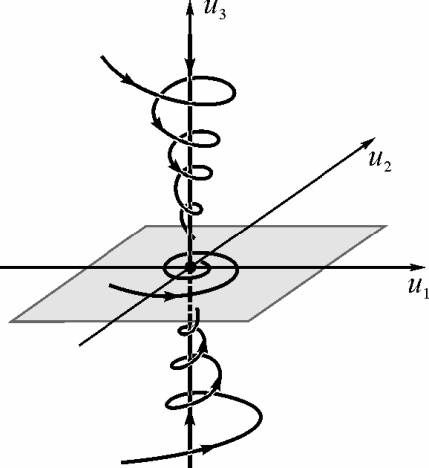
\includegraphics[]{fig/lect4/4a}

                (a)
        \end{minipage}
        \begin{minipage}{0.45\linewidth}
                \centering  
                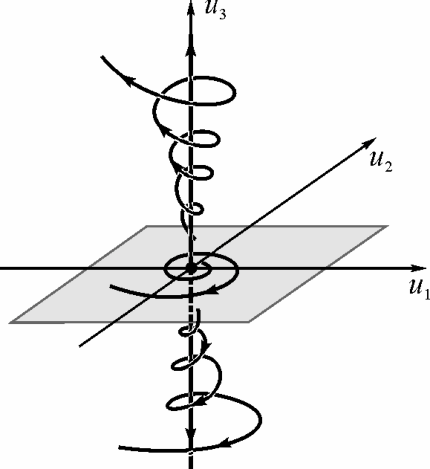
\includegraphics[]{fig/lect4/4b}

                (b)      
        \end{minipage}
        \caption{Состояние равновесия системы \eqref{eq:4.18}: устойчивый фокус (a); 
        неустойчивый фокус (b).}
        \label{fig:4.4}
\end{figure}

\paragraph{Случай $\Re \lambda_{1,2}>0$ и $\lambda_3>0$.}%
\label{par:sluchai_re_1,2_0_i_lambda_3_0_}

Поведение траекторий системы \eqref{eq:4.18} при таких характеристических показателях можно легко установить, сделав в системе замену $t \to - t$. Такая замена сводит данный случай к предыдущему.
Следовательно, искомый фазовый портрет подобен портрету, представленному на рис.\ref{fig:4.4}а, в котором надо лишь изменить направление движения по траекториям на противоположное. Полученное состояние равновесия называется неустойчивым фокусом (см. рис.\ref{fig:4.4}b).

\subsubsection{Вещественные части корней $\lambda_i$ разных знаков}%
\label{ssub:veshchestvennye_chasti_kornei_lambda_i_raznykh_znakov}

\paragraph{Случай $\Re \lambda_{1,2}<0$ и $\lambda_3>0$.}%
\label{par:sluchai_re_1,2_0_i_lambda_3_0_}

При этих условиях двумерное многообразие $E^{s} = \qty{ u_3 =0, ~ (u_1, u_2) \in \R^2}$ является устойчивым, а двумерное $E^{u} = \qty{u_1 = u_2=0, u_3 \in \R}$ -- неустойчивым.
На многообразии $E^{s}$ система \eqref{eq:4.18} имеет устойчивый двумерный фокус, а $E^{u}$ состоит из двух неустойчивых сепаратрис $E_1^{u}, E_2^{u}$ и точки $O$. Принимая во внимание неравенство \eqref{eq:4.19}, устанавливаем, что все траектории, вне многообразий $E^{s}$ и $E^{u}$,
асимптотически приближаются к прямой $E^{u}$, удаляясь при этом от состояния равновесия. Фазовый портрет такого состояния равновесия представлен на рис.\ref{fig:4.5}а. Оно называется седло-фокусом.

\paragraph{Случай $\Re \lambda_{1,2}>0$ и $\lambda_3<0$}%
\label{par:sluchai_re_1,2_0_i_lambda_3_0_}
Обратив в системе \eqref{eq:4.18} время $t \to - t$, мы получим рассмотренный выше случай. Поэтому для построения фазового портрета изучаемого состояния равновесия достаточно просто изменить на рис.\ref{fig:4.5}а направление движения по траекториям на противоположное. В результате получится состояние равновесия, представленное на рис.\ref{fig:4.5}b, которое также называется седло-фокусом. Однако, у этого состояния равновесия неустойчивым является двумерное многообразие, а устойчивым -- одномерное многообразие.

\begin{figure}[h!]
        \centering
        \begin{minipage}{0.45\linewidth}
                \centering  
                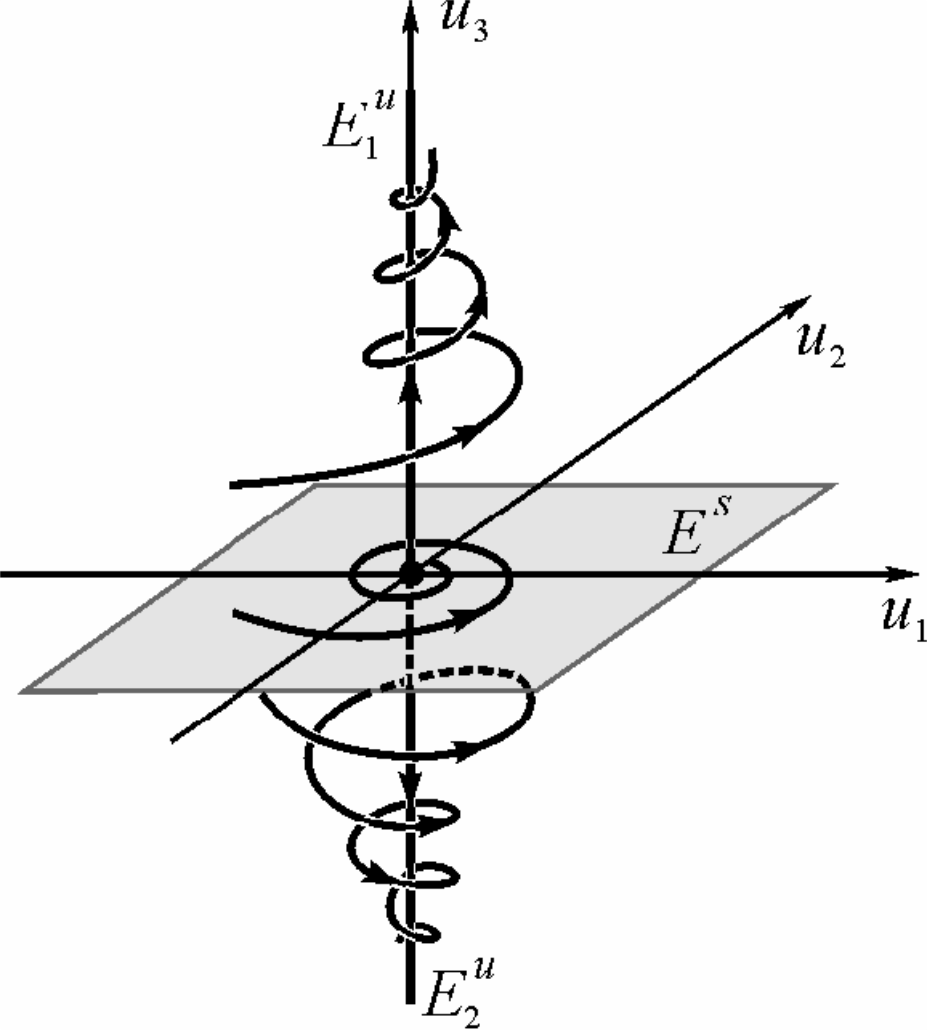
\includegraphics[]{fig/lect4/5a}

                (a)
        \end{minipage}
        \begin{minipage}{0.45\linewidth}
                \centering  
                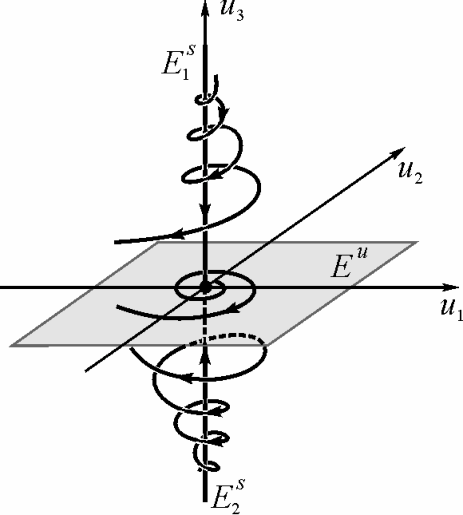
\includegraphics[]{fig/lect4/5b}

                (b)      
        \end{minipage}
        \caption{Состояние равновесия системы \eqref{eq:4.18}: седло-фокус с двумерным устойчивым и одномерным неустойчивым многообразиями (а); седло-фокус с двумерным неустойчивым и одномерным устойчивым многообразиями (b)}
        \label{fig:4.5}
\end{figure}


\subsection{Состояния равновесия трехмерных нелинейных систем}%
\label{sub:sostoianie_ravnovesiia_trekhmernykh_nelineinykh_sistem}

Рассмотрим поведение траекторий нелинейной трехмерной системы \eqref{eq:4.1} в
окрестности состояния равновесия. Если состояние равновесия является
грубым 
$\qty(\Re \lambda_i \neq 0,~ i=1,2,3)$ , то существует непрерывное взаимно-однозначное
отображение, имеющее непрерывное обратное отображение, под действием
которого каждая траектория из окрестности состояния равновесия нелинейной
системы \eqref{eq:4.1} переводится в траекторию из окрестности состояния равновесия
линеаризованной системы с сохранением направления движения (теорема
Гробмана-Хартмана). Следовательно, структура окрестности состояния
равновесия нелинейной системы качественно выглядит также как окрестность
состояния равновесия соответствующей линеаризованной системы. При этом
размерность и устойчивость многообразий линеаризованной и нелинейной
систем совпадают. Однако, многообразия нелинейной системы представляют
собой, вообще говоря, некоторые поверхности и кривые, а не плоскости и
прямые, как в случае линеаризованной системы. Инвариантные многообразия
состояния равновесия нелинейной системы касаются в этом состоянии
равновесия многообразий линеаризованной системы (теорема Адамара-Перрона)
\paragraph{Пример}%
\label{par:primer}

\begin{equation}
        \label{eq:4.20}
        \begin{cases}
                \dot x = x - y^2 - z^2, \\
                \dot y = - y, \\
                \dot z = - z.
        \end{cases}
\end{equation}
Система \eqref{eq:4.20} имеет единственное состояние равновесия - $O(x=y=z=0)$  характеристическими показателями: $\lambda_3=1, \lambda_2=-1,, \lambda_1=-1$. Следовательно, $O$ -- седло. Нетрудно видеть, что многообразия седла линеаризованной системы имеют вид
\begin{gather}
        E^s = \qty{ x=0, ~ (y,z)} \in \R^2\\
                E^{u} = \qty{ y =z =0 ,~ x} \in \R.
\end{gather}
С другой стороны, непосредственно из \eqref{eq:4.20} следует, что неустойчивое многообразие $W^u$ седла $O$ системы \eqref{eq:4.20} совпадает с прямой $E^u$, а устойчивое многообразие $W^s$ задается следующим образом
\begin{equation}
        \label{eq:}
        W^s = \qty{ x = \frac{y^2}{3} + \frac{z^2}{5} }.
\end{equation}
Качественный вид многообразий седла иллюстрирует рис.\ref{fig:4.6}, который ясно показывает принципиальное 
различие инвариантных многообразий нелинейных и линеаризованных систем. Заметим, что совпадение $W^u$ и $E^u$ в системе \eqref{eq:4.20} носит частный характер и не отражает общей ситуации. 

\begin{figure}[h!]
        \centering
        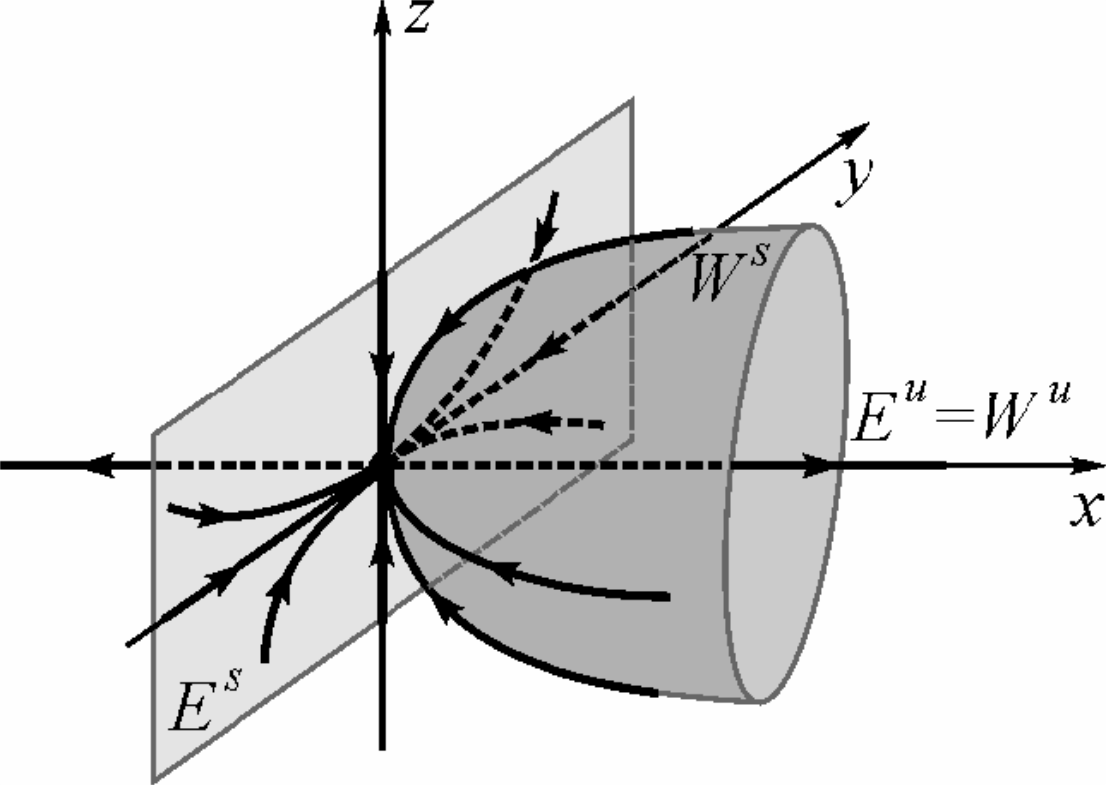
\includegraphics[width=0.6\linewidth]{fig/lect4/6}
        \caption{Многообразие линеаризованной -- $E^s,~E^u$ и нелинейной системы \eqref{eq:4.20} --$W^s,~ W^u$.}
        \label{fig:4.6}
\end{figure}

В заключение этого раздела обратим внимание на то, что утверждения, сформулированные выше, относительно свойств состояний равновесия трехмерных систем имеют соответствующие аналоги и для систем произвольной размерности.

\subsection{Двухпараметрическая бифуркационная диаграмма}%
\label{sub:4.4.4}

Характеристическое уравнение \eqref{eq:4.10} содержит три параметра $a,b$ и $c$, от значения которых зависит расположение корней этого уравнения на комплексной плоскости и, следовательно, тип состояния равновесия $O$. Установим связь между параметрами $a,b,c$ и характером состояния равновесия. Согласно результатам, изложенным в разделах \ref{sec:4.2} и \ref{eq:4.4}, разбиение пространства параметров $\qty{a,b,c}$ на области, соответствующие различным типам состояний равновесия  $O$ определяется следующими условиями  
\begin{equation}
        \label{eq:4.21}
        a=0, ~ ab-c=0,~ c=0,~ D=0,
\end{equation}
где $D$ -- дискриминант уравнения \eqref{eq:4.10}, имеющий вид
\begin{equation}
        \label{eq:}
        D = \frac{b^3}{27} - \frac{a^2b^2}{108} + \frac{a^3c}{27} - \frac{abc}{6} + \frac{c^2}{4}.
\end{equation}
Уравнение \eqref{eq:4.10} имеет действительные корни, если $D<0$ и один действительный и два комплексно-сопряженных корня, если $D>0$. При $D=0$ корни уравнения \eqref{eq:4.10} действительные, два из которых равны между собой. Зафиксируем параметры и рассмотрим двухпараметрическую задачу, считая $b$ и $c$ контрольными параметрами.

\paragraph{Случай $a=\const >0.$}%
\label{par:sluchai_a_const_0_}

Из условий \eqref{eq:4.21} следует, что разбиение плоскости $(b,c)$ (см. рис.\ref{fig:4.7})
на области, соответствующие различным типам состояний равновесия осуществляется следующими буфуркационными кривыми 
\begin{gather}
        C^{\pm} = \qty{ c = \frac{ a(9b-2a^2) \pm 2(a^2-3b)^{\frac{3}{2}}}{27},~ b<\frac{a^2}{3}},\\
        S = \qty{ c= ab, ~ b>0}, ~ B^+ = \qty{c=0, b> \frac{a^2}{4}} \\
        B^0 = \qty{c=0, ~ 0<b<\frac{a^2}{4} }, B^- =\qty{c=0,~b<0}.
\end{gather}

\begin{figure}[h!]
        \centering
        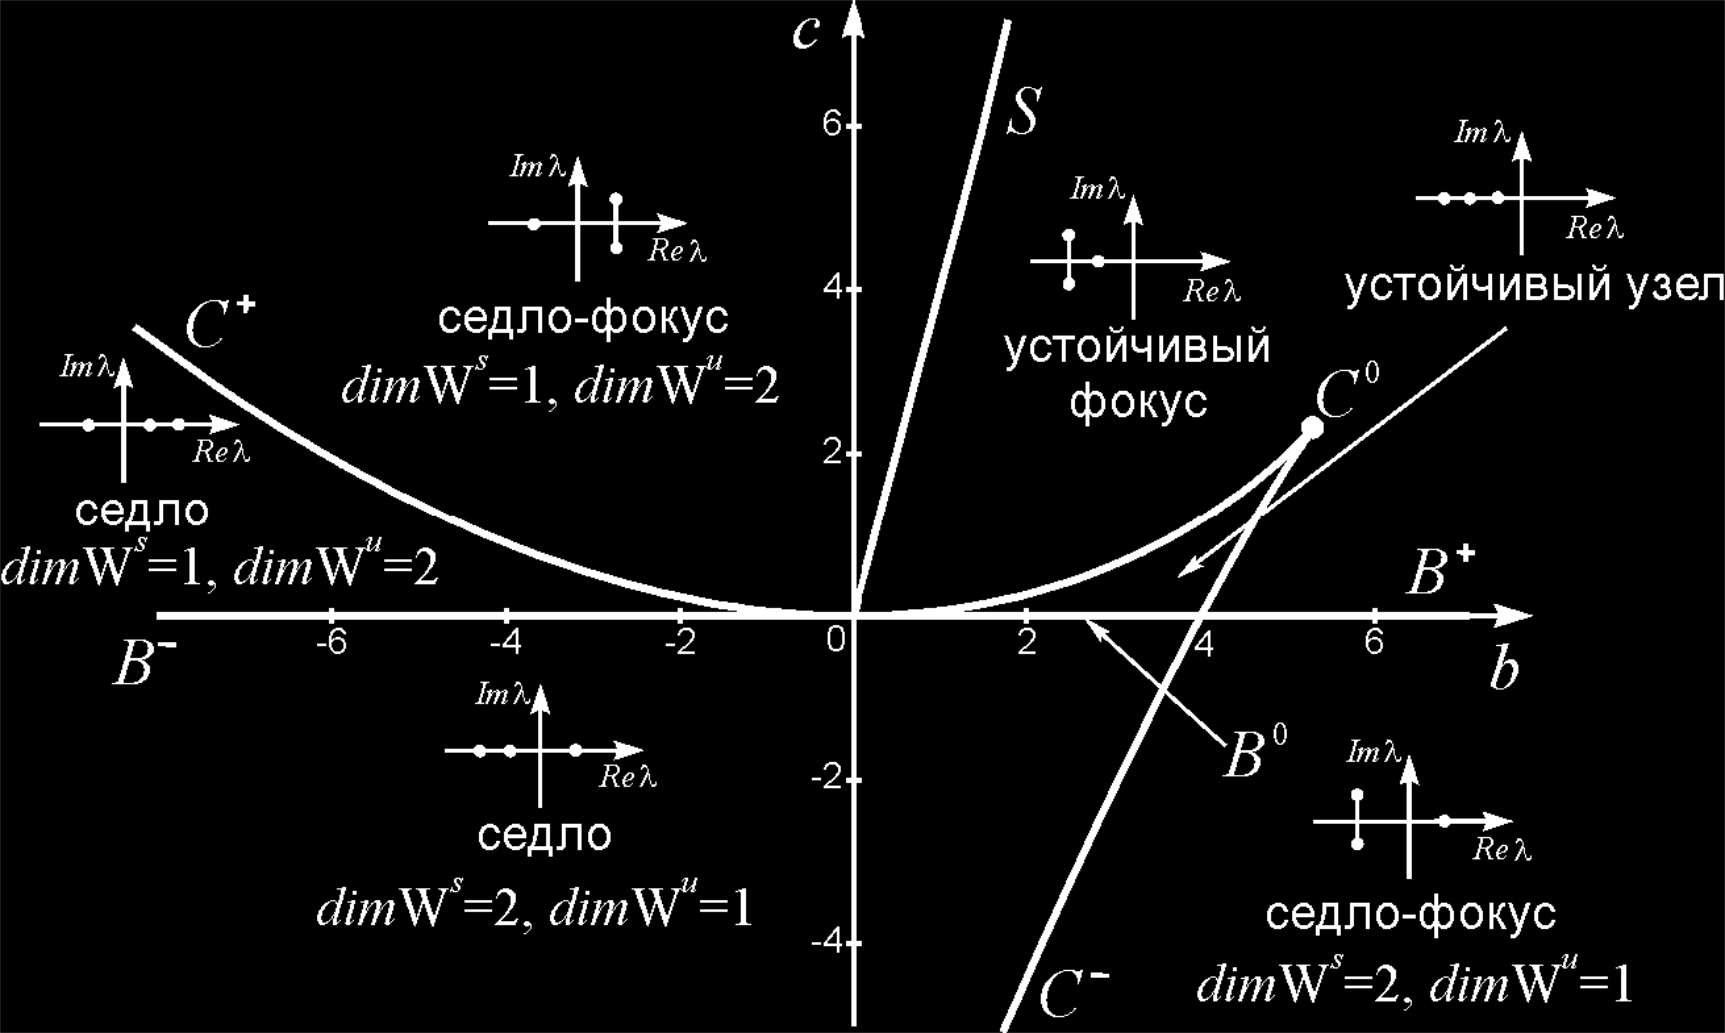
\includegraphics[width=0.6\linewidth]{fig/lect4/7}
        \caption{Разбиение плоскости параметром $(b,c)$ на области, соответствующие различным типам состояния равновесия систему \eqref{eq:4.4} в случаях $a>0 ~ (a=4)$.}
        \label{fig:4.7}
\end{figure}

\paragraph{Случай $a=0$.}%
\label{par:sluchai_a_0_}
При $a=0$ область асимптотической устойчивости отсутствует, отрезок $B^0$ стягивается в точку -- начало координат, а кривые $C^+$ и $C^-$ целиком расположены в области $b<0$ (см. рис.\ref{fig:4.8}). В этом случае на полупрямой $B^+$ уравнение \eqref{eq:4.10} имеет, кроме одного нулевого, ещё пару чисто мнимых корней, а в начале координат -- трехкратный нулевой корень. На плоскости $(b,c)$ существует четыре области, соответствующие различным типам грубого состояния равновесия $O$. 

\paragraph{Случай $a<0$.}%
\label{par:sluchai_a_0_}

Как и при $a>0$, здесь разбиение плоскости $(c,b)$ на области, соответствующие различным типам состояния равновесия, осуществляют бифуркационные линии $C^{\pm},~S,~B^{\pm}$ и $B^0$ (см. рис.\ref{fig:4.9}). Однако, расположение корней уравнения \eqref{eq:4.10} на комплексной плоскости, когда параметры принадлежат $B^+, ~ B^0$ и $S$ отличается от случая $a>0$. Именно точкам полупрямай $B^+$ отвечает один нулевой и два комплексно-сопряженных корня с положительной вещественной частью, отрезка $B^0$ - один нулевой и два положительных корня, а полупрямой $S$ -- один положительный  и  два чисто мнимых корня. Изменился также и вид кривых $C^+$ и $C^-$. Кривая $C^+$ стала монотонно убывающей
и выпуклой вниз, а $C^-$ -- выпуклой вверх, имеющей максимум в начале координат. При $a<0$ состояние равновесия всегда неустойчиво по Ляпунову и на плоскости $(b,c)$ существуют шесть областей, отвечающих различным типам состояния равновесия $O$.

\begin{figure}[h!]
        \centering
        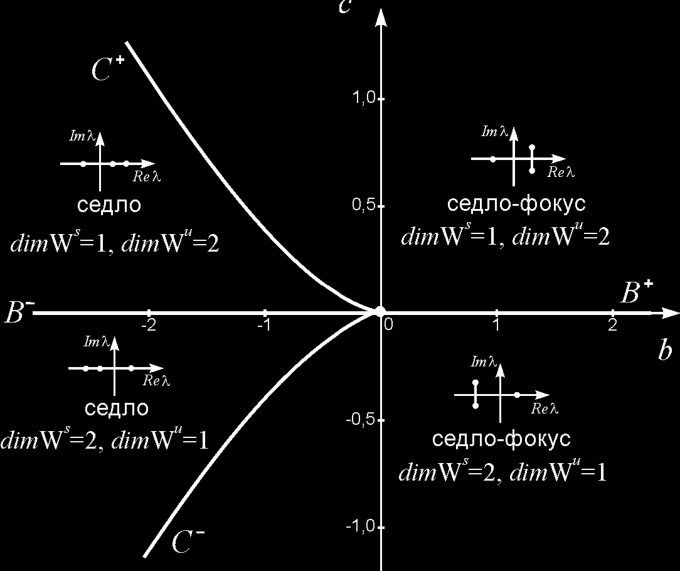
\includegraphics[width=0.5\linewidth]{fig/lect4/8}
        \caption{Разбиение плоскости параметров $(b,c)$ на области, соответствующие различным типам состояния равновесия системы \eqref{eq:4.4} в случае $a=0$.}
        \label{fig:4.8}
\end{figure}

\begin{figure}[h!]
        \centering
        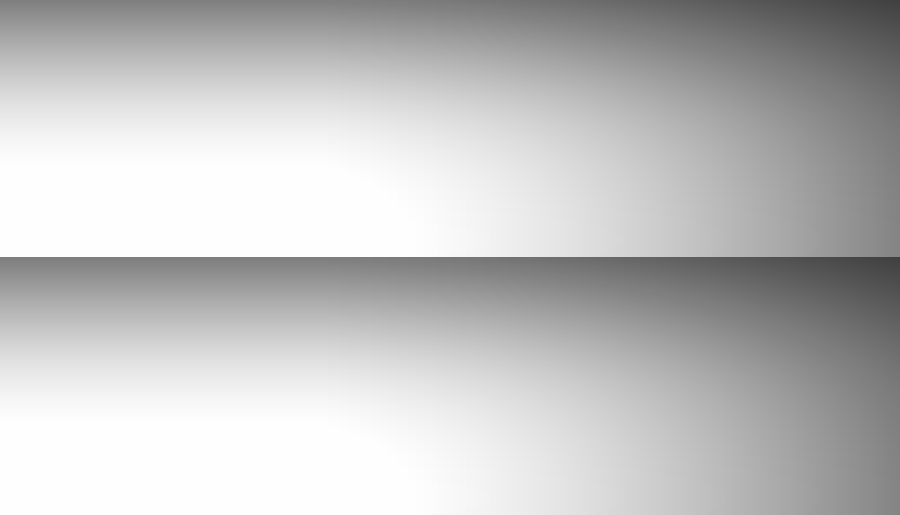
\includegraphics[width=0.5\linewidth]{fig/lect4/9}
        \caption{Разбиение плоскости $(b,c)$ на области, соответствующие различным типам состояния равновесия \eqref{eq:4.4} в случае $a<0$ $(a=-4)$.}
        \label{fig:4.9}
\end{figure}


